\section{IMU基本模型}

惯性测量单元(inertial measurement unit,以下简称IMU),是测量物体三轴角速度以及加速度的装置。IMU工作极其稳定,几乎不会有宕机的情况,而且通常能以远高于相机的频率(数百到上千赫兹)得到相对于自身坐标系的角速度$\bm\omega$($rad \cdot s^{-1}$)和加速度$\mathbf{a}$($m \cdot s^{-2}$)。依靠这些数据,我们可以通过计算得到系统的旋转、速度和平移信息。很自然地,由于IMU工作并不依赖于视觉信息,它可以在恶劣的光照、纹理以及模糊图像的条件下为我们提供可靠的跟踪结果。并且我们注意到,整个系统的速度$\mathbf{v}$和平移$\mathbf{p}$分别来自于加速度$\mathbf{a}$的一次和二次数值积分,因此基于IMU的跟踪结果直接就带有了场景的尺度信息。

然而正确地使用IMU并不是一件容易的事情。和所有传感器一样,IMU信号也带有误差,不管是使用滤波的方法还是非线性优化的方法处理IMU信息,我们都要对其进行合理的建模。我们可以将IMU的输出数据(IMU对实际运动的观测)和输入数据(实际的物理运动)的差异定义为IMU读数的误差,它可能包含偏移\footnote{bias,指IMU输出值和输入值之间的偏移,可能受温度、重力等因素的影响}、随机游走噪声\footnote{random walk,指当输入固定时,IMU输出值中包含的随机噪声,它随时间的变化可被认为是一个随机过程}、尺度系数\footnote{scale factor,指的是输出和输入之间相差的一个倍数}、不正交性\footnote{non-orthogonality,指由于IMU各轴并不完全正交所带来的误差}等等\citep{imu2014}。如图\ref{fig:common_imu_errors}展示了一种常见的IMU误差模型。

\begin{figure}[htb!]
    \centering
    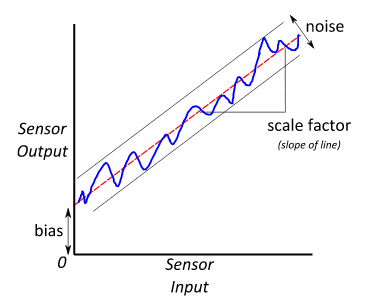
\includegraphics[width=.4\textwidth]{./figs/common_imu_errors.png}
    \caption{一般的IMU误差模型\citep{imu2014}}
    \label{fig:common_imu_errors}
\end{figure}

可以看到,IMU误差的成分是比较复杂的,不同类型误差对于运动估计的影响也是不同的。前面我们提到,在位姿估计的过程中,我们会对角速度$\bm\omega$进行数值积分,得到系统的朝向$\mathrm{R}$,而对加速度$\mathbf{a}$进行一次和二次积分,分别得到速度$\mathbf{v}$和平移$\mathbf{p}$。加速度经过了两次数值积分,其误差也会通过两次积分进入平移量$\mathbf{p}$中,故相比角速度的误差,我们的跟踪算法对于加速度的误差更为敏感。实际经验也告诉我们,由IMU积分得到的朝向信息是较为准确的,而位置信息的误差则是较大的。

不过,一般IMU在出厂时都会经过厂商的校准,故我们可以不必使用上面那样复杂的误差模型。以常用的六轴IMU为例,目前VIO算法中最为常用的做法是将其误差模型简化为偏移和测量噪声两个部分,并假设加速度计和陀螺仪相互统计独立,且各自的三轴之间都统计独立。我们用下标$m$标记每次观测的值,不带下标的表示真实值,在不考虑地球自转的情况下,角速度和加速度的观测量分别为\citep{mourikis2007multi}:

\begin{equation}
\begin{aligned}
    \tilde{\bm\omega} &= \bm\omega + \mathbf{b}^g + \bm\eta^g,  \\
    \tilde{\mathbf a} &= \prescript{G}{}{\mathrm{R}^\top}
                         (\prescript{G}{}{\mathbf a} - \prescript{G}{}{\mathbf g}) +
                         \mathbf{b}^g + \bm\eta^g
\end{aligned}
\end{equation}

使用左上标$^G$来表示全局坐标系,不带左上标的表示当前的局部坐标系。可以看到,IMU的的读数可以看成是真实值、偏移和加性高斯白噪声(addative Gaussian white noise)之和。加速度计又有点特殊,它的读数里面还包含重力$\prescript{G}{}{\mathbf g}$的影响。

另外就是所谓的偏移和白噪声了:
\begin{itemize}
    \item 偏移$\mathbf{b}$随时间的增长符合零均值的高斯随机游走。这个噪声从IMU开机以来就一直存在,不断积累,与是否从IMU读取数据无关。可以用一个初始偏移量$\mathbf{b}_0$和随机游走噪声$\mathbf{n}_w$来描述它:$\mathbf{b} = \mathbf{b}_0 + \mathbf{n}_b$;
    \item 测量噪声$\bm\eta$为零均值的加性高斯白噪声,表示从IMU读取数据时产生的小抖动,而且这个噪声只在观测它的时候产生。
\end{itemize}

其中:

\begin{equation}
\begin{aligned}
    \mathbf{n}_{bg} & \thicksim \mathcal{N}(\mathbf{0}, \mathrm\Sigma_{bg}), &
    \bm\eta_{wg}    & \thicksim \mathcal{N}(\mathbf{0}, \mathrm\Sigma_{wg}), \\
    \mathbf{n}_{ba} & \thicksim \mathcal{N}(\mathbf{0}, \mathrm\Sigma_{ba}), &
    \bm\eta_{wa}    & \thicksim \mathcal{N}(\mathbf{0}, \mathrm\Sigma_{wa}),
\end{aligned}
\end{equation}

故它们的协方差矩阵为:

\begin{equation}
    \mathrm{Q}_{\textrm{IMU}} = \mathbf{diag}(
        \mathrm\Sigma_{bg},
        \mathrm\Sigma_{wg},
        \mathrm\Sigma_{ba},
        \mathrm\Sigma_{wa}
    )
\end{equation}

\subsection{离散时间噪声和连续时间噪声}

上面说的噪声模型都是在连续时间系统下面考虑的,连续时间系统的高斯协方差(或标准差)也就称为传感器的噪声强度。实际上我们不可能每时每刻都在观测IMU,这是一个离散时间系统。离散时间噪声和连续时间噪声的关系,可以参考\citep{smith1978exact}。这里我们只是简单地给出离散时间系统下噪声的协方差。以陀螺仪为例,一般我们会假设我们会假设三轴的噪声独立同分布,假设采样时间间隔为$\Delta t$,那么陀螺仪的两种噪声协方差就是:

\begin{equation}
\begin{aligned}
    \mathrm\Sigma_{bgd} &= \mathrm\Sigma_{bg} \Delta t,  \\
    \mathrm\Sigma_{wgd} &= \mathrm\Sigma_{wg} / \Delta t.
\end{aligned}
\end{equation}

加速度计的形式是一样的。

\subsection{IMU状态传递}

所谓的IMU状态传递(IMU propagation)指的就是根据通过将当前时刻IMU的读数在时间上进行积分,来得到下一时刻的IMU状态。这个IMU状态包括IMU的位姿、运动以及噪声等,通过积分操作,IMU读数的信息就被“传递”到了下一时刻。

我们先来考虑理想情况,也就是IMU的读数不存在白噪声,偏移量也不存在随机游走的情况,此时IMU的读数符合:

\begin{equation}
\begin{aligned}
    \bm\omega  &= \tilde{\bm\omega} - \mathbf{b}^g, \\
    \mathbf{a} &= \tilde{\mathbf a} - \mathbf{b}^a + \mathbf{g}.
\end{aligned}
\end{equation}

记全局坐标系下IMU的状态为(为保持简洁,省略了转置符号${}^\top$):

\begin{equation}
  \mathbf{X}_{\textrm{IMU}} \triangleq
  \left[
      \prescript{G}{}{\mathrm R},
      \prescript{G}{}{\mathbf p},
      \prescript{G}{}{\mathbf v},
      \mathbf{b}^g, \mathbf{b}^a
  \right].
\end{equation}

具体来说,积分过程包括积分这个IMU状态向量的五个分量。那么,要对IMU状态进行积分,我们首先要写出IMU状态关于时间的导数:

\begin{equation}
\begin{aligned}
    \prescript{G}{}{\dot{\mathrm R}}
        &= \prescript{G}{}{\mathrm R} \lfloor(\tilde{\bm\omega} - \mathbf{b}^g)\times\rfloor, \\
    \prescript{G}{}{\dot{\mathbf p}}
        &= \prescript{G}{}{\mathbf v}, \\
    \prescript{G}{}{\dot{\mathbf v}}
        &= \prescript{G}{}{\mathrm R} (\tilde{\mathbf a} - \mathbf{b}^a + \mathbf{g}), \\
    \dot{\mathbf b}^g &= \mathbf{0}, \\
    \dot{\mathbf b}^a &= \mathbf{0}
\end{aligned}
\end{equation}

显然,由于偏移$\mathbf{b}^g$和$\mathbf{b}^a$随时间的增长符合零均值的高斯随机游走,故它们关于时间的导数为零。积分的步骤如下:

\begin{enumerate}
    \item 将角速度在时间上积分,得到当前IMU的朝向;
    \item 将加速度在时间上积分,得到当前IMU的速度;
    \item 将速度再在时间上积分,得到当前IMU的位置;
    \item 角速度偏移和加速度偏移由于增长符合零均值随机游走,所以直接取旧的状态中的值。
\end{enumerate}

我们可以使用任意一种数值积分算法来实现,比如欧拉法(Euler method)、龙格库塔法(Runge-Kutta methods)\citep{wiki2017runge}等。此外,不仅要对状态向量进行数值积分,同时我们还要更新协方差矩阵。
